\section{Marco teórico}

En esta sección se presenta el desarrollo llevado a cabo para lograr los objetivos propuestos, haciendo énfasis en los aspectos teóricos que fundamentan el proyecto.

Para poder utilizar un transformador pequeño y cumplir con las especificaciones normalmente se requieren conversiones de etapas múltiples.
Las fuentes de potencia otorgan una alta densidad de potencia en un tamaño y con un peso reducido.  
Además, permiten aislar eléctricamente a la carga de la red de alimentación. 
%Dirección controlada del flujo de potencia. 
%Alta eficiencia de conversión. 
Utilizando filtros simples es posible tener formas de onda con baja distorsión armónica tanto en la entrada como en la salida. 
%Permiten controlar el factor de potencia si la fuente es de AC. %Que cosa? Los filtros?

En base a la tensión de salida requerida existen fuentes de alimentación AC y fuentes de alimentación DC.
Las fuentes de alimentación DC se clasifican en:
\begin{description}
    \item[Conmutadas]
    Tienen una alta eficiencia y pueden suministrar altas corrientes de carga a una tensión baja.
    Existen 5 topologías comunes: fly-back, forward, push–pull, half-bridge, y full-bridge.
    Por lo general se utilizan 2 etapas de conversión: DC-AC mediante modulación de ancho de pulso (PWM) de la etapa del inversor y de AC-DC.
    La salida del inversor, que varía mediante una señal PWM, se convierte en un voltaje DC mediante un rectificador de diodos. 
    Debido a que el inversor puede operar a una frecuencia muy alta, las fluctuaciones en la tensión de salida de DC se pueden filtrar fácilmente.
    \item[Resonantes]
    Si la variación del voltaje de salida no es amplia se pueden usar inversores de pulso resonante. 
    La frecuencia del inversor, que podría ser la misma que la frecuencia de resonancia, es muy alta y la tensión de salida del inversor es casi sinusoidal 
    Debido a la oscilación resonante, el núcleo del transformador siempre se restablece y no hay problemas de saturación. 
    Los tamaños del transformador y del filtro de salida se reducen debido a la alta frecuencia del inversor.
    \item[Bidireccionales]
    Aptas para carga y descarga de baterías donde el flujo de potencia es bidireccional. 
    Este último depende de la tensión de entrada, de la tensión de salida y de la relación de vueltas del transformador. 
    Permiten que la corriente inductiva fluya en cualquier dirección y que el flujo de corriente se vuelva continuo.
    Requiere sintetizar las funciones de conmutación para obtener las formas de onda de salida deseadas.
\end{description}

% Especificaciones de la tensión de salida del prototipo: 12.6VDC
Para seleccionar una topología adecuada para una aplicación, es necesario comprender las ventajas y desventajas de cada topología y los requisitos de la aplicación. 
Existen diversas topologías, las cuales serán analizadas en orden creciente de complejidad. 
Aunque la mayoría de los convertidores se pueden utilizar para cumplir con los requerimientos de salida, 
los valores nominales del dispositivo de conmutación y el tamaño del transformador limitan sus aplicaciones a una potencia de salida específica. 
La elección del convertidor depende del requisito de potencia de salida y de la complejidad que se desea afrontar.

\subsection{Convertidor Forward}

Es un convertidor CC-CC acoplado magnéticamente. El transistor funciona como interruptor, estará cerrado un tiempo $DT$ y abierto el resto del tiempo,
$(1 - D)T$, siendo $T$ el periodo de conmutación. 
El transformador posee tres devanados: los devanados 1 y 2 transfieren la energía de la
fuente a la carga cuando el interruptor está cerrado; el devanado 3 se usa para proporcionar un
camino a la corriente magnetizante cuando el interruptor está abierto y reducirla a cero antes del
inicio de cada periodo de conmutación. El transformador se modela como tres devanados ideales
con una inductancia magnetizante $L_m$ conectada en paralelo con el devanado 1. En este modelo simplificado no se incluyen las pérdidas ni las inductancias de dispersión.
En el convertidor forward, $L_m$ es un parámetro no incluido en la relación entrada-salida y se suele adoptar un valor grande.

A diferencia del convertidor flyback, la energía del generador se transfiere a la carga cuando el interruptor
está cerrado. En el convertidor flyback, la energía se almacena en el primario cuando el conmutador
está cerrado y se transfiere a la carga cuando está abierto. 
La eficiencia se incrementa reestableciendo el núcleo del transformador, 
donde la energía almacenada en el mismo es devuelta a la fuente de entrada del convertidor a partir del tercer bobinado. 
Además, sólo se opera en el modo de conducción continua por la mayor dificultad del control en base al doble polo existente en el filtro de salida. 

% REVISAR NOMENCLATURA EN BASE A LAS IMÁGENES A UTILIZAR DE LOS LIBROS
Asumiendo modo de conducción continua, operación en estado estacionario, ripple de salida nulo 
y que la corriente en la inductancia del filtro de salida $L_x$ es permanente, existen 2 modos de operación del transistor:

% RASHID EN INGLÉS

\paragraph{Cuando el transistor se encuentra encendido}

En la Figura $X$ se muestra el circuito equivalente del convertidor forward cuando el interruptor
está cerrado. Al cerrarse el interruptor se establece una tensión en el primer devanado del transformador,
lo cual induce tensiones en el segundo y tercer devanado:

% HART INGLÉS PÁGINA 279 DEL LIBRO 
$$ v_1=V_s $$
$$ v_2=v_1\left(\frac{N_2}{N_1}\right)=V_s\left(\frac{N_2}{N_1}\right) $$
$$ v_3=v_1\left(\frac{N_3}{N_1}\right)=V_s\left(\frac{N_3}{N_1}\right) $$

La tensión v2 positiva polariza en directa a D1 y en reversa a D2. El diodo D3 no conduce ya que su tensión es negativa:

$$ V_{D_3}=-V_s-v_3<0 $$

La tensión en la bobina es:
% vlx
$$ v_{L_x}=v_2-V_0=V_s\left(\frac{N_2}{N_1}\right)-V_o=L_x\frac{di_{L_x}}{dt} $$

Reorganizando los términos obtenemos:
% ecuación de abajo
$$ \frac{di_{L_x}}{dt}=\frac{V_s(N_2/N_1)-V_o}{L_x}=\frac{\Delta i_{L_x}}{\Delta t}=\frac{\Delta i_{L_x}}{DT} $$

Como la derivada de la corriente es una constante positiva, la corriente aumenta linealmente. 
La variación de corriente cuando el interruptor está cerrado se calcula modificando la ecuación anterior:
% ecuación de abajo 7-22
$$ (\Delta i_{L_x})_{closed}=\left[V_s\left(\frac{N_2}{N_1}\right)-V_o\right]\frac{DT}{L_x} $$

La tensión en la inductancia magnetizante es igual a la tensión en el primario del transformador, por lo cual:
% ecuación 7-23
$$ \Delta i_{L_m}=\frac{V_sDT}{L_m} $$

La corriente que circula por el transistor está compuesta por:
% ecuación 7-24
$$ i_{sw}=i_1+i_{L_m} $$

% FIN HART INGLÉS PÁGINA 279 DEL LIBRO

La corriente que circula por el primario comienza a incrementarse,
se transfiere energía del primario al secundario y de aquí al filtro de salida y la carga por medio del diodo D2 polarizado en directa. 
Debido a esta corriente se induce una corriente en el secundario dada por:
% RASHID INGLÉS PÁGINA 666 DEL LIBRO 
$$ i_p=\frac{N_s}{N_p}i_{se} $$

Por lo tanto, 
% ESCRIBIR iprimario=f(isecundario)  (al reves que antes)
$$ i_p=f(i_{se}) $$

La corriente magnetizante se incrementa linealmente con el tiempo:

$$ i_{mag}=\frac{V_s}{L_m}t $$

La corriente total que circula por el primario resulta:

$$ i_p'=i_p+i_{mag}=\frac{N_s}{N_p}i_{se}+\frac{V_s}{L_m}t $$

Cuando finaliza el tiempo de conducción del transistor en un tiempo $t=DT$, esta corriente llega a un valor máximo dado por:

$$ I_{p_{max}}'=I_{p_{max}}+\frac{V_sDT}{L_m} $$

donde $I_{p_{max}}$ es la corriente pico reflejada a la salida del inductor $L_x$ y está dada por:

$$ I_{p_{max}}=\frac{N_p}{N_s}I_{L_{1_{max}}} $$

Debido a la tensión $V_{se}-V_o$ existente en bornes del inductor de salida, su corriente se incrementa linealmente:

$$ \frac{di_{L_x}}{dt}=\frac{V_s-V_o}{L_x} $$

Esta misma también tendrá su valor máximo en $t=DT$:

$$ I_{L_{1_{max}}}=I_{L_x}(0)+\frac{(V_s-V_o)DT}{L_x} $$

\paragraph{Cuando el transistor se encuentra apagado}
En la figura \ref{fig:forward_switch_open} se muestra el circuito equivalente del convertidor forward cuando el interruptor está abierto. 
Las tensiones de todos los bobinados del transformador toman polaridad negativa, lo cual apaga al diodo $D_1$ y enciende a los diodos $D_2$ y $D_3$. 
La corriente magnetizante y la corriente en el inductor del filtro de salida no pueden cambiar instantáneamente cuando el transistor se apaga. 
La continuidad de $i_{L_m}$ establece $ i_1=-i_{L_m} $
% SACAR DEL TEXTO INICIAL

\begin{figure}[ht]
    \centering
    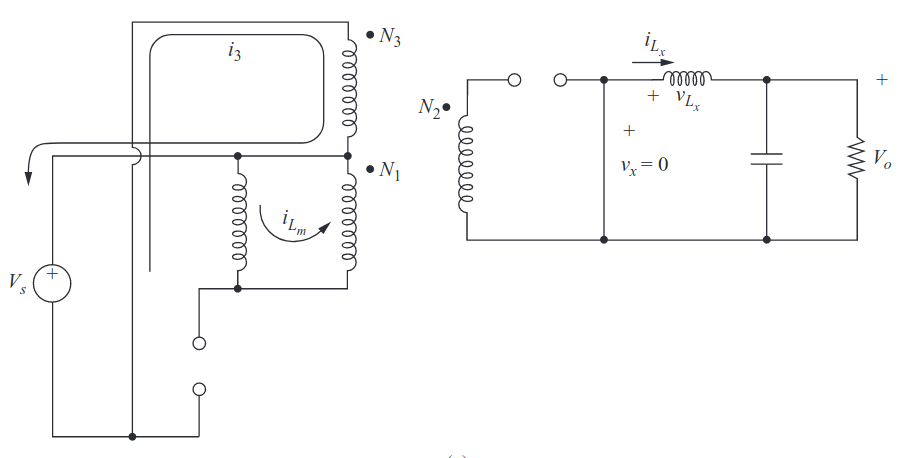
\includegraphics[width=0.8\textwidth]{../images/hart/forward_switch_open.png}
    \caption{}
    \label{fig:forward_switch_open}
\end{figure}

La corriente que sale del terminal con punto homólogo del primer bobinado quiere establecer una corriente que ingresa al terminal 
con punto homólogo del segundo bobinado, pero el diodo D1 no permite la circulación de la corriente en esa dirección. 
Además, la corriente que sale del terminal con punto homólogo del primer bobinado induce una corriente que ingresa al terminal 
con punto homólogo del tercer bobinado. Esto polariza en directa al diodo $D_3$, a la vez que 
se le provee a la corriente magnetizante de un camino a través del tercer bobinado de regreso a la fuente de entrada. 

Con D3 encendido, la tensión en el tercer bobinado resulta:
% HART EN INGLES PÁGINA 280 DEL LIBRO 
$$ v_3=-V_s $$

Esto induce las siguientes tensiones en los otros bobinados:
% ECUACIÓN 7.25
$$ v_1=v_3\left(\frac{N_1}{N_3}\right)=-V_s\left(\frac{N_1}{N_3}\right) $$
$$ v_2=v_3\left(\frac{N_2}{N_3}\right)=-V_s\left(\frac{N_2}{N_3}\right) $$

Con $D_1$ apagado y corriente positiva en el inductor de salida, $D_2$ se polariza en directa. 
Mientras conduce $D_2$, la energía es entregada a la carga a través del inductor de salida. 
La tensión sobre la misma resulta:
% ECUACIÓN 7.26
$$ v_{L_x}=-V_o=L_x\frac{di_{L_x}}{dt} $$

Reorganizando los términos obtenemos:

$$ \frac{di_{L_x}}{dt}=\frac{V_o}{L} $$

Como la derivada de la corriente es una constante negativa, la corriente disminuye linealmente. 
La variación de corriente cuando el interruptor está abierto se calcula modificando la ecuación anterior:

$$ (\Delta i_{L_x})_{open}=\frac{-V_o(1-D)T}{L_x} $$

La corriente por el inductor y el diodo $D_2$ es la misma y decrece linealmente con el tiempo:
%% RASHID (13.19)
$$ i_{L_x}=i_{D_3}=I_{L_{x_{max}}}-\frac{V_o}{L_x}t,\ 0<t\leq (1-k)T $$

Lo cual nos da el valor de $I_L(t=0)=i_{L_x}(t=(1-k)T)=I_{L_{x_{max}}}-V_o(1-k)T/L_x$
%% RASHID POST (13.19)

En estado estacionario el cambio neto en la corriente del inductor durante un período debe ser cero:
% ECUACIÓNES PRE 7.27
$$ (\Delta i_{L_x})_{closed}+(\Delta i_{L_x})_{open}=0 $$
$$ \left[V_s\left(\frac{N_2}{N_1}\right)-V_o\right]\frac{DT}{L_x}-\frac{V_o(1-D)T}{L_x}=0 $$

Resolviendo se obtiene la tensión de salida:
% ECUACIÓN 7.27
$$ V_o=V_sD\left(\frac{N_2}{N_1}\right) $$

La tensión en la inductancia magnetizante es igual a la tensión en el primario del transformador, la cual decrece linealmente con el tiempo:
% ECUACIÓN 7.28 Y 7.29
$$ v_{L_m}=v_1=-V_s\left(\frac{N_1}{N_3}\right)=L_m\frac{di_{L_m}}{dt} $$

$$ \frac{di_{L_m}}{dt}=-\frac{V_s}{L_m}\left(\frac{N_1}{N_3}\right) $$

$$ \frac{\Delta i_{L_m}}{\Delta t}?-\frac{V_s}{L_m}\left(\frac{N_1}{N_3}\right) $$ 

Se puede observar que el diodo $D_3$ impide que la corriente $i_{L_m}$ se haga negativa. 

% VER DONDE PONER ESTAS 2 ECUACIONES
%% RASHID (13.21) Y (13.22)
La máxima corriente de colector se da durante el encendido del transistor y la máxima tensión de colector durante el apagado:

$$ I_{C_{max}}=I_{p_{max}}'=\left(\frac{N_p}{N_s}\right)I_{L_{x_{max}}}+\frac{V_sDT}{L_m} $$
$$ V_{Q_{1_{max}}}=V_{s_{max}}+V_{r_{max}}=V_{s_{max}}\left(1+\frac{N_p}{N_r}\right) $$

Para que el flujo magnético vuelva a 0, la corriente magnetizante debe anularse al final de cada ciclo de conmutación, desmagnetizando el núcleo del transformador.
Para lograrlo, el decrecimiento de la corriente debe ser igual a su incremento dado por la variación de corriente cuando el interruptor está cerrado. 
Si el tiempo necesario para que la corriente $i_{L_m}$ se anule desde su valor máximo es $\Delta T_x$, 
% ECUACIÓN 7.30
$$ \frac{\Delta i_{L_m}}{\Delta T_x}=-\frac{V_sDT}{L_m}=-\frac{V_s}{L_m}\left(\frac{N_1}{N_3}\right) $$

Resolviendo para obtener $\Delta T_x$,
% ECUACIÓN 7.31
$$ \Delta T_x=DT\left(\frac{N_3}{N_1}\right) $$

El instante $t_0$ en el que se anula la corriente es:
% ECUACIÓN 7.32
$$ t_0=DT+\Delta T_x=DT+DT\left(\frac{N_3}{N_1}\right)=DT\left(1+\frac{N_3}{N_1}\right) $$

Teniendo en cuenta que la corriente debe anularse antes del inicio del siguiente periodo,
% ECUACIÓN 7.33
$t_0<T$

$$ sDT\left(1+\frac{N_3}{N_1}\right)<T $$

$$ D\left(1+\frac{N_3}{N_1}\right)<1 $$

Para evitar la saturación del núcleo del transformador, el ciclo de trabajo debe mantenerse siempre por debajo del máximo.
El transistor puede dañarse si el núcleo se satura.

La tensión en el interruptor abierto es $V_s-v_1$, por lo que
% ECUACIÓN 7.34
$$
v_{sw}=
\begin{cases}
    V_s-v_1=V_s-\left(-V_s\frac{N_1}{N_3}\right)=V_s\left(1+\frac{N_1}{N_3}\right) & \text{para $DT<t<t_0$}\\
    V_s & \text{para $t_0<t<T$}
\end{cases}
$$

% FIN HART EN ESPAÑOL PÁG 272

% HART EN ESPAÑOL PÁG 208

La configuración del circuito a la salida del convertidor forward es la misma que la del convertidor
reductor, por lo que el rizado de la tensión de salida también será el mismo:

$$  $$

Rizado de la tensión de salida

En el análisis anterior hemos supuesto ripple de salida nulo, es decir, que el capacitor de salida era muy grande para que la tensión
de salida fuese constante. En la práctica no será posible mantener perfectamente constante la
tensión de salida con una capacidad finita. La variación periódica de la tensión de salida, o rizado,
se calcula a partir de la relación entre la tensión y la corriente del capacitor. 
La corriente en el capacitor es:

$$  $$

Dicha corriente se muestra en la Figura X. El capacitor se cargará mientras sea positiva la corriente en el mismo. Aplicando la definición
de capacidad,

$$  $$

$$  $$

$$  $$

La variación de la carga, DELTAQ, es el área del triángulo situado por encima del eje de tiempos:

$$  $$

Reemplazando:

$$  $$

Sustituyendo el valor de la variación de corriente en la bobina cuando el interruptor está abierto, 
se obtiene la tensión de rizado pico a pico en la salida, mostrada en la Figura X.

$$  $$

Si el rizado no es muy grande, la suposición de que la salida es constante es razonable, y el
análisis anterior será válido.

% FIN HART EN ESPAÑOL PÁG 209

En resumen, cuando el interruptor está cerrado, la fuente entrega energía a la carga a través del transformador.
La tensión en el secundario del transformador es una forma de onda pulsante. La energía almacenada en
la inductancia magnetizante cuando el interruptor está cerrado es devuelta a la fuente de
entrada a través de un tercer devanado del transformador cuando el interruptor está abierto.

\subsection{Comparación con el convertidor flyback}

El convertidor forward requiere de una carga mínima para evitar un exceso en la tensión de salida. 
Como el transformador no almacena energía, para un mismo nivel de potencia de salida, 
el tamaño del mismo es menor en el convertidor forward que en el flyback. 
La corriente de salida es aproximadamente constante ya que el ripple disminuye notablemente 
debido al agregado del inductor en la salida y al diodo de rueda libre D1.
Por esto mismo, el capacitor de salida puede ser más pequeño. 

\subsection{Convertidor Forward Doble Switch}

El convertidor forward se utiliza para potencias de salida de hasta 200W ya que se encuentra limitado 
por los esfuerzos de tensión y corriente a los que se somete el transistor de potencia durante su funcionamiento. 
El convertidor forward de doble switch puede ser utilizado con potencias de hasta 750W. 
A partir de los diodos D3 y D4 en el primario, se reduce la tensión de colector en los transistores cuando los mismos 
se encuentran apagados, lo cual permite utilizar transistores de menores prestaciones.

\subsubsection{Funcionamiento}

Los transistores se encienden y se apagan de forma simultánea, lo cual los diferencia de las topologías bridge. 
Cuando los transistores están encendidos, la tensión en el primario del transformador es igual a la tensión de entrada $V_s$. 
En consecuencia, la tensión en el devanado secundario es positiva y la energía se transfiere a la carga. 
Además la corriente que circula por la inductancia magnetizante se incrementa con el tiempo. 

Cuando los transistores se apagan, el diodo D1 evita que la corriente magnetizante circule por el secundario 
(y por lo tanto también en el primario) del transformador, forzando su camino por los diodos D3 y D4 de regreso a la fuente de entrada.  
Con esto se elimina la necesidad del tercer devanado de desmagnetización. 
La tensión en el primario del transformador es $-V_s$, causando un decremento en el tiempo de la corriente magnetizante. 
Si la relación de trabajo de los transistores es menor a 0.5, en cada ciclo el núcleo del transformador se restablece.
La tensión de salida es la misma que la del convertidor forward con un interruptor descrito anteriormente.
La principal ventaja de esta topología es que la tensión de colector en los transistores cuando los mismos se encuentran apagados 
es $V_s$ y no $V_s\left(1+\frac{N_1}{N_3}\right)$ como en el forward de un único switch.

\subsection{Circuitos de control}

La tensión de salida del convertidor puede ser controlada variando el ciclo de trabajo D. 
Para ello se utilizan circuitos integrados controladores PWM que sólo requieren de unos pocos componentes pasivos adicionales para su funcionamiento. 
Internamente presenta 4 componentes principales:
\begin{enumerate}
    \item Un reloj ajustable que permite configurar la frecuencia de conmutación
    \item Amplificador de error para la tensión de salida
    \item Generador de forma de onda de dientes de sierra sincronizado con el reloj
    \item Un comparador para comparar la señal de salida de error con la señal de dientes de sierra
\end{enumerate}

La señal de salida del circuito PWM es la que controla a los transistores. 

Para controlar la tensión de salida, los convertidores funcionan con un circuito de retroalimentación,
dependiendo de la señal realimentada, en un control por tensión o corriente. En la figura \ref{fig:marco_teorico:control} se muestra un diagrama de bloques del circuito.

\begin{figure}[ht]
    \centering
    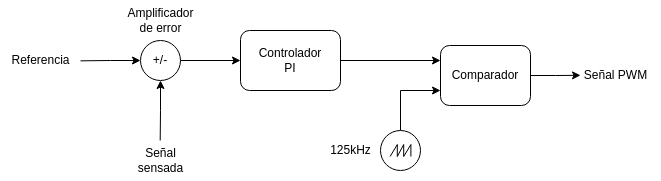
\includegraphics[width=0.8\textwidth]{images/compensador.png}
    \caption{Diagrama de bloques del circuito de control}
    \label{fig:marco_teorico:control}
\end{figure}

\subsubsection{Control por tensión}

%COMPLETAR CON LIBRO
El bloque de control mide la tensión a la salida del convertidor, la escala y la compara con la tensión deseada.
Esto genera una señal de error, la cual alimenta a un controlador PI.

La duración del tiempo de encendido está determinada por el tiempo entre el reinicio del generador de diente de sierra
y la intersección del voltaje de error con la señal de rampa positiva. 
Cuando la tensión de salida es inferior al valor nominal se genera una tensión de error. 
El ciclo de trabajo aumenta para causar un aumento posterior en el voltaje de salida. 
La dinámica de retroalimentación está determinada por el circuito amplificador de error que consta de Z1 y Z2.

\subsubsection{Control por corriente}

Consiste en un lazo interno que muestrea el valor de la corriente primaria y apaga los interruptores tan pronto como la corriente alcanza cierto valor establecido por el lazo de voltaje externo. 
De esta manera, el control de corriente logra una respuesta más rápida que el modo de voltaje. 
La forma de onda de corriente primaria actúa como onda de diente de sierra. 
la tensión análoga a la corriente puede ser proporcionada por una pequeña resistencia o por un transformador de corriente. 
La figura 13.19a muestra un convertidor flyback controlado por modo de corriente, donde la corriente del interruptor isw se usa como señal portadora. 
La corriente del interruptor isw produce un voltaje a través de Rs, que se retroalimenta al comparador. 
El encendido está sincronizado con el pulso del reloj y el apagado está determinado por el instante en que la corriente de entrada es igual al voltaje de error.
Debido a su capacidad inherente de limitación de corriente máxima, el control de modo de corriente puede mejorar la confiabilidad de los interruptores de alimentación. El rendimiento dinámico se mejora debido al uso de la información actual adicional. El control de modo de corriente reduce efectivamente el sistema a primer orden al obligar a que la corriente del inductor se relacione con el voltaje de salida, logrando así una respuesta más rápida. Las figuras 13.18b–e muestran las formas de onda.

% COMPLETAR CON JUSTIFICACIÓN DE POR QUÉ NO ELEGIMOS CONTROL POR CORRIENTE QUE PARECERÍA SER MEJOR. 

\subsubsection{TL494}

El TL494 es un circuito de control de modulación de ancho de pulso (PWM) de frecuencia fija. 
La modulación de los pulsos de salida se logra comparando la forma de onda de diente de sierra creada por el oscilador interno en el capacitor de temporización (CT) con cualquiera de las dos señales de control. 
La etapa de salida se habilita durante el tiempo en que el voltaje de diente de sierra es mayor que las señales de control de voltaje. 
A medida que aumenta la señal de control, disminuye el tiempo durante el cual la entrada en diente de sierra es mayor; por lo tanto, la duración del pulso de salida disminuye. 
Un flip-flop de dirección de pulso dirige alternativamente el pulso modulado a cada uno de los dos transistores de salida.

Alimentación: 7-40V.
El TL494 está diseñado para operar desde un rango de suministro de voltaje de entrada entre 7 V y 40 V.

Feedback: sin conexión ya que se trabaja a lazo abierto

Regulador interno de 5V con precisión del 5\%. 

Oscilador interno ajustable:
Provee la forma de onda de diente de sierra al tiempo muerto y al comparador PWM. 
Su frecuencia se programa mediante la selección de una resistencia Rt y un capacitor Ct. 
El oscilador carga al Ct con una corriente constante determinada por Rt produciendo una rampa de tensión sobre Ct.
$$ I_{carga}=\frac{3V}{R_t} $$
Cuando la tensión sobre el mismo llega a 3V, el circuito se descarga y se reinicia el ciclo. 
$f=\frac{1}{R_t\cdot C_t}$ para single ended 
Según la hoja de datos, los valores recomendados para Rt y Ct son:
$$470pF\leq C_t\leq 10\mu F$$
$$1.8k\Omega\leq R_t\leq 500k\Omega$$
Para lograr la $f=125kHz$ se eligió un capacitor de $1nF$ y para lograr la resistencia de $8k\Omega$ se ajustó un potenciómetro de $10k\Omega$. 

Control de tiempo muerto (DTC):
Permite controlar el ciclo de trabajo. 
Es una entrada de alta impedancia. 
Controla el tiempo de apagado mínimo. Con DTC a tierra es del 3\%.
Si se aplica tensión en este puerto se le puede adicionar.
El tiempo muerto o de apagado se controla linealmente desde su mínimo de 3\% hasta su máximo de 100\%, 
variando su tensión de entrada entre 0 y 3.3V respectivamente. 

Comparador:
Alimentado por el regulador interno. 
Tiempo de respuesta de $400ns$. 
Modula el ancho de pulso de la salida. Para esto se compara la rampa de tensión sobre el capacitor $C_t$ con la señal de control
presente en la salida de los amplificadores de error. 

Dos amplificadores de error:
Presentan alta ganancia y se alimentan mediante su entrada $V_i$. 
Tensión de MC de entrada: -0.3V a $V_{cc}-2V$

Output-Control Input:
Determina el modo de operación de la salida de los transistores. 
Si está a tierra opera en modo single-ended o modo paralelo donde los pulsos vistos en la salida del DTC son transmitidos por ambos transistores de salida en paralelo.
Si está a Vref opera en push-pull donde cada transistor de salida está habilitado alternativamente por el flip-flop de dirección de pulsos.

Transistores de salida:
El integrado incluye 2 transistores que tienen la posibilidad de ser emisor común o seguidor por emisor. 
Son capaces de generar hasta $200mA$ de salida. 

% REVISAR SI ES DEL TL494 O ES UNA NOTA AL TUN TUN
% Transformador: permite que no circule corriente continua por su secundario. 

\subsubsection{Amplificador Clase B con transistores complementarios}

Sin esta etapa de amplificación, dado que la carga que generaba el circuito sobre el TL494 era muy alta, 
la forma de onda PWM se distorsionaba y disminuía su amplitud notablemente, lo que causaba que los MOSFETs no se saturaran y aumentaran demasiado su temperatura.
Los resultados obtenidos con la inclusión de esta etapa fueron un incremento notorio en la amplitud y una mejora en la forma de onda de la señal PWM.

La etapa permite acoplar la carga en continua. 
Los transistores utilizados son de potencia y no de señal. 
Cada dispositivo de amplificación conduce durante medio ciclo de la señal de entrada, 
excitándolos mediante el ingreso de corriente por su base.

Se compone de un transistor NPN y otro PNP que se alimentan de forma inversa.
El transistor NPN requiere de una tensión positiva en su colector y 
el transistor PNP requiere de una tensión negativa en su colector.
Ambos funcionan como seguidor por emisor o colector común, con su tensión de alimentación en colector, la señal de excitación en la base y la carga conectada el emisor. 
Su ganancia de tensión es aproximadamente 1. 
La topología seguidor por emisor tiene ganancia de corriente hfe. 
La corriente que se entrega por la base es hfe veces menor que la que se le entrega a la carga. 
El seguidor presenta una impedancia de entrada es mucho mas alta que su impedancia de salida, de modo que una fuente de señal no tendría que trabajar tan duro.
 Esto puede verse en el hecho de que la corriente de base es del orden de 100 veces menos que la corriente de emisor. 
 La baja impedancia de salida del seguidor emisor se adapta con una carga de baja impedancia y amortigua la fuente de señal.

Los transistores conducen en base a la tensión Vbe en sus junturas ya que entra base y emisor existe una juntura PN similar a un diodo. 
Si no se polariza de forma correcta, no circula corriente por su base y en consecuencia tampoco por su colector. 
El transistor NPN conduce corriente en su emisor cuando $V_{be}>0$. 
El transistor PNP conduce corriente en su emisor cuando $V_{be}<0$ o $V_{eb}>0$.
En el semiciclo positivo de la señal conduce el NPN y el PNP se corta y en el semiciclo negativo conduce el PNP y el NPN se corta. 
Los transistores conducen de forma alternativa. 
Cuando la tensión de entrada en la base de ambos transistores es 0 no conduce ningún transistor. 
Esto implica que no existe consumo de corriente ni de potencia. 
La Vce de ambos transistores va de $V_{cc}$ a 0.

\subsection{Snubber}

Un circuito snubber o de amortiguación es una red RC que permite eliminar ruido de alta frecuencia que existe en los nodos de los transistores.
Hasta ahora se ha analizado el convertidor forward sin tener en cuenta los elementos parásitos asociados a cada componente. 
Algunos ejemplos de estos son la resistencia serie equivalente e inductancia serie equivalente de los capacitores, 
la capacidad parásita de los transistores o la resistencia e inductancia parásita de las conexiones realizadas. 
La energía acumulada en las inductancias parásitas mientras los transistores conmutan provoca una resonancia con el capacitor de filtrado en la entrada. 
La red snubber conforma un camino de baja impedancia para el drenaje de esta energía. 
Valores pequeños de estos elementos parásitos generan resonancias del orden de los MHz. 

\subsubsection{Funcionamiento}

La energía acumulada en las inductancias parásitas mientras los transistores están encendidos se almacena como energía electroestática en el capacitor de la red snubber Csnb. 
Cuando los transistores conducen, su tensión se eleva hasta Vin, la energía almacenada en el capacitor es: 
$$ E=0.5\times C_{snb}V_{in}^{2} $$
La carga eléctrica del capacitor luego de su carga es:
$$ Q=C_{snb}V_{in} $$
La potencia suministrada por la fuente de entrada en cada ciclo es:
$$ V_{in}Q=C_{snb}V_{in}^{2} $$
Las pérdidas en la resistencia $R_{sbn}$ resultan:
$$ P_{R_{snb}}=C_{snb}V_{in}^{2}f_{sw} $$
Durante la carga mitad de esta potencia se consume en la resistencia Rsnb por efecto Joule y la otra mitad se almacena en el capacitor Csnb. 
Cuando los transistores no conducen, su tensión disminuye hasta 0V, toda la energía almacenada se descarga y es consumida en la resistencia de amortiguamiento $R_{snb}$.
Cuando se descarga, mitad de la energía almacenada se convierte en calor en la resistencia $R_{snb}$. 
El análisis supone que el tiempo de carga y descarga es mucho más grande que la constante de tiempo RC. 

\subsubsection{Procedimiento para el cálculo de los componentes}

\begin{enumerate}
    \item Con el osciloscopio se mide la frecuencia de la oscilación en la tensión del transistor Vds. $f_{r}=1.27MHz$ %Era esa?
    \item Se conecta un capacitor entre Drain y Source con una capacidad $C_{p_{0}}$ tal que la frecuencia de la oscilación disminuya a la mitad. $C_{p_{0}}=$
    \item La frecuencia de resonancia en una red LC está dada por
    $$ w=\frac{1}{\sqrt{LC}} $$
    Con la configuración actual, 
    $$ f_{r}=\frac{1}{2\pi\sqrt{L_{p}(C_{p_{2}}+C_{p_{0}})}} $$
    Para lograr que dicha frecuencia disminuya a la mitad se necesita una capacitancia total que sea cuatro veces la capacitancia parásita con la que se comenzó.
    Por lo tanto, la capacidad parásita del circuito resulta un tercio de la capacidad agregada. $C_{p_{2}} = \frac{C_{p_{0}}}{3}$
    \item Teniendo la capacidad parásita del circuito Cp2 y la frecuencia de la oscilación original se puede calcular la inductancia parásita del circuito:
    $$ L_{p}=\frac{1}{(2\pi f_{r})^{2}*C_{p_{2}}} $$
    \item La impedancia característica de los elementos parásitos resulta:
    $$ Z_{0}=\sqrt{\frac{L_p}{C_{p_2}}} $$
    \item El valor óptimo para la $R_{snb}$ es aproximadamente igual a la impedancia característica. Debe ser mayor o igual a esta última. Un valor muy alto puede permitir un pico propio de la oscilación y un valor más bajo permite una corriente más elevada, resultando en un sobrecalentamiento.
    \item Se elige una Csnb que sea igual o hasta 4 veces superior a la capacidad parásita del circuito. $C_{p_2}\leq C_{snb}\leq 4C_{p_2}$
    \item Se calcula la potencia disipada en Rsnb y se utiliza una resistencia cuya potencia máxima sea el doble que la disipada.
    $$ P_{R_{snb}}=C_{snb}V_{in}^2f_{sw} $$
    \item Se agrega un capacitor de Bypass de 0.1uF para amortiguar la inductancia del MOSFET high side.     
\end{enumerate}